\documentclass[twocolumn]{article}
\usepackage[spanish]{babel}
\usepackage{caption}
\usepackage{graphicx}
\usepackage{amsmath}
\setlength{\parindent}{0pt}

\author{Josué Villasante}
\title{Medición del tamaño de spot de un laser}

\begin{document}
	\maketitle

	\section{Objetivo}
		El objetivo fue obtener el tamaño del spot del láser a partir del cambio de intensidad a medida el láser es bloqueado por el filo de una cuchilla perpendicular al haz.
	
	\section{Motivación}
		Al analizar la potencia de entrada y de salida del haz del láser a través de una fibra óptica se observó que aproximadamente solo el 30\% lograba atravesar. El lente del coalimador no es el correcto para el láser que tenemos. Por lo tanto, es necesario medir el tamaño del spot del láser a fin de poder conocer cuál es el lente correcto.
	
	\section{Procedimiento}
		El láser utilizado tuvo una longitud de onda de 633nm y una potencia menor a 20mW. Primero se colocó la cuchilla a aproximadamente unos 30cm del láser y se bloqueo completamente el haz. El potenciometro se colocó a 50cm del láser. Luego, por cada movimiento de 0.1mm se registró la intensidad del láser en mW. Al iniciar, la base marcaba 5mm.

		El mismo procedimiento de realizó colocando la cuchilla a un distancia de 1m del laser y el potenciometro a 1.1m.

	\section{Resultados}
		Para el primer caso a 30cm del láser las mediciones obtenidas fueron las siguientes.

		\begin{center}
			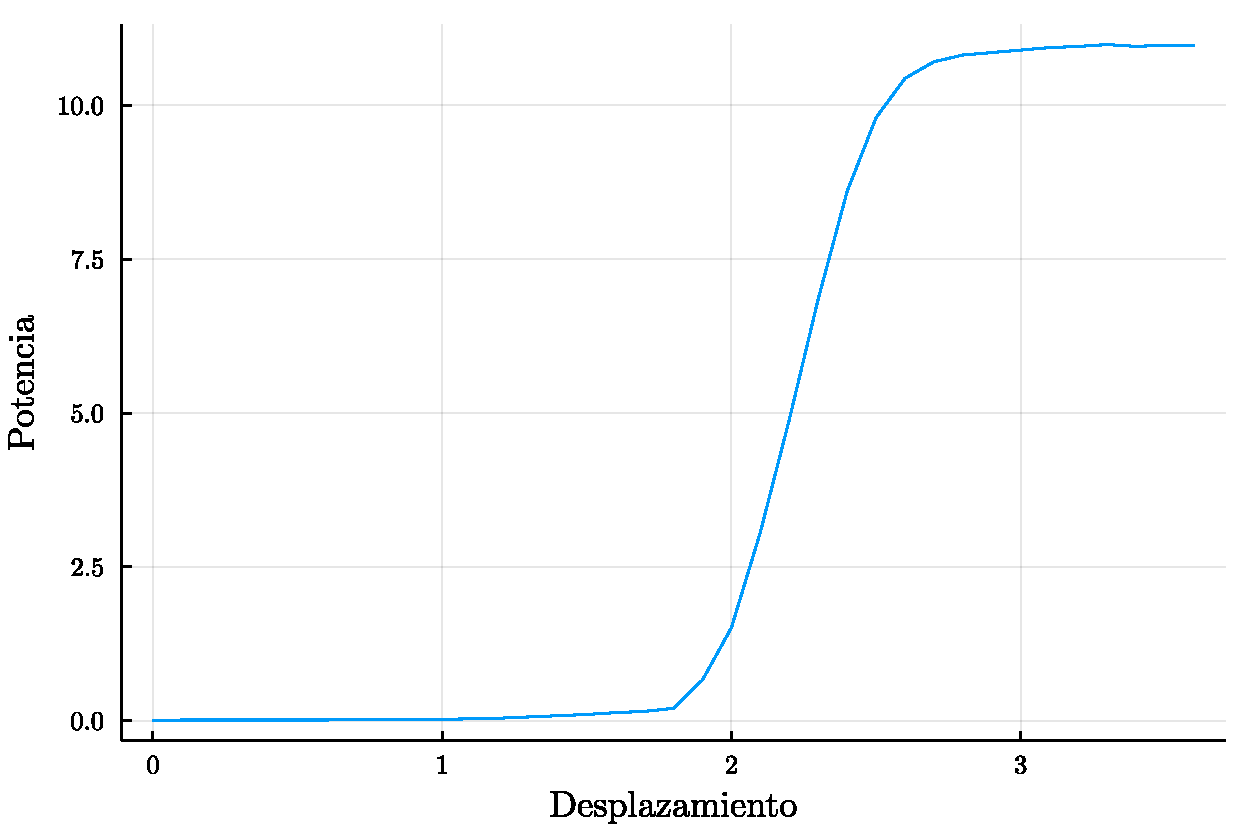
\includegraphics[width=200pt]{img/measurement_1.pdf}
			\captionof{figure}{Potencia según desplazamiento de la cuchilla a 30cm del láser}
		\end{center}

		El segundo caso arrojó los siguientes resultados.

		\begin{center}
			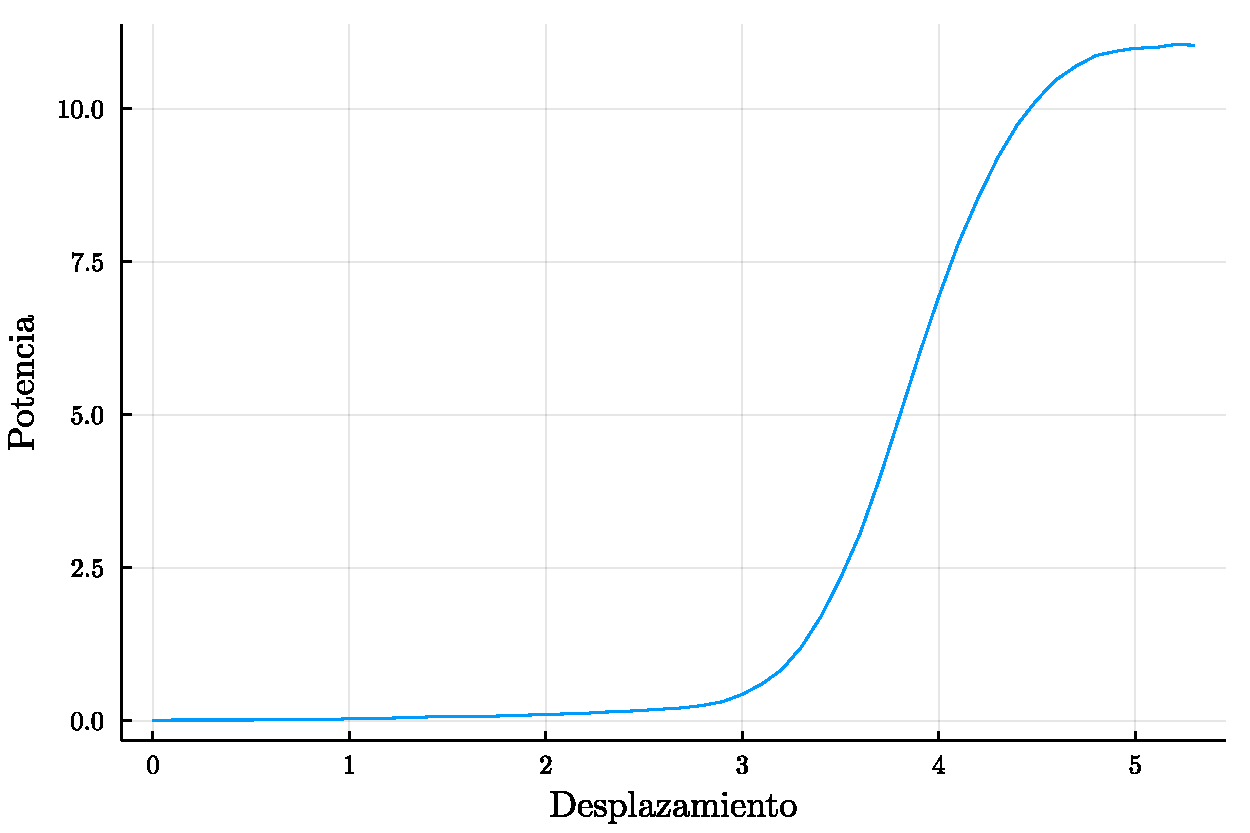
\includegraphics[width=200pt]{img/measurement_2.pdf}
			\captionof{figure}{Potencia según desplazamiento de la cuchilla a 1m cm del láser}
		\end{center}

		Por otro lado, se sabe que la distribución de la potencia del spot del laser es normal, y por lo tanto puede ser descrita por la siguiente función dado los valores de $\mu$ y $\sigma$.
		
		$$
		f(x) = \frac{1}{\sigma\sqrt{2\pi}}\exp({-\frac{1}{2}(\frac{x-\mu}{\sigma})^2})
		$$

		Entonces para encontrar el tamaño del spot se ajustó
		$$\int{f(x)dx}$$
		a los datos encontrados para así encontrar los valores de $\mu$ y $\sigma$. Para esto se utilizó el algoritmo de Levenberg-Marquardt y se encontró los siguientes valores para la primera medición.

		$$
		\sigma = 0.2180458 \
		$$
		$$
		\mu = 2.2313830
		$$

		Tomando estos valores se evaluó la función dónde $f(x) = \frac{1}{e^2}$.

		\begin{center}
			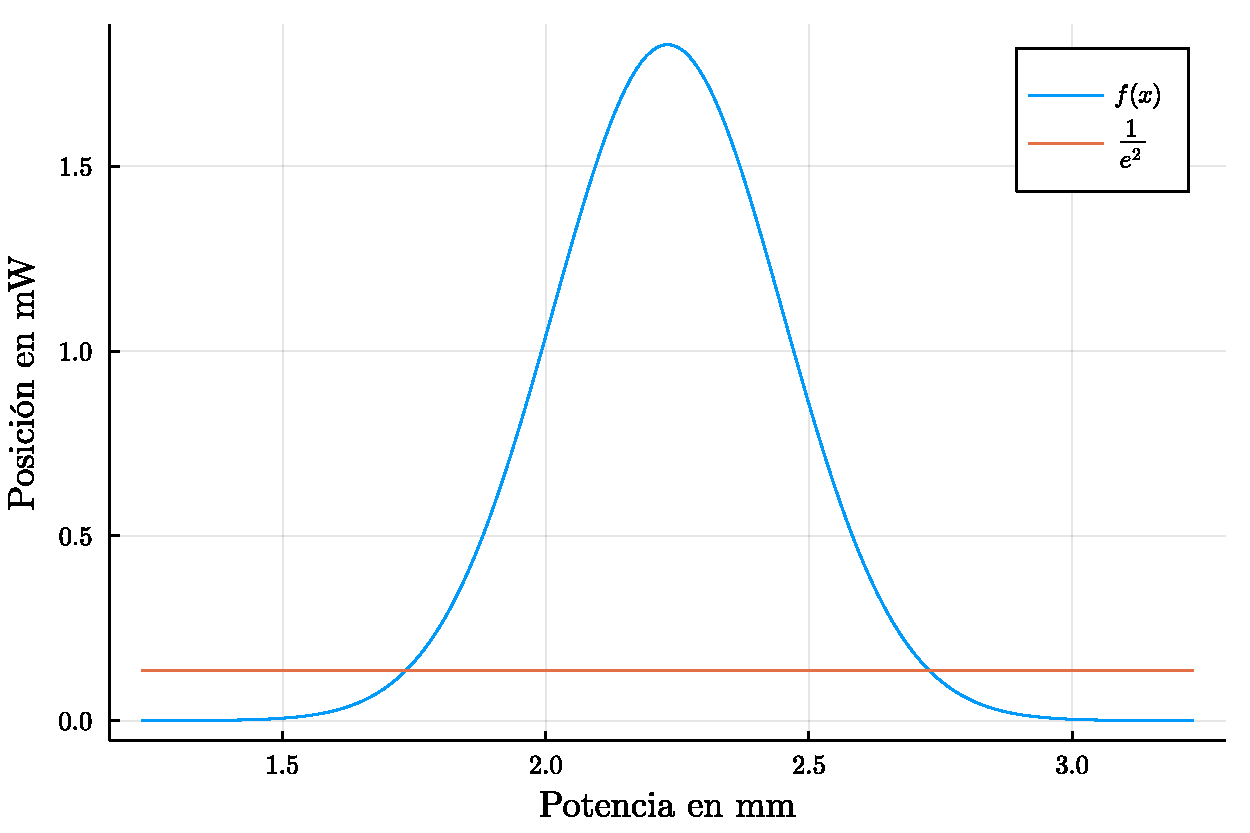
\includegraphics[width=200pt]{img/normal_1.pdf}
			\captionof{figure}{Potencia en función de la posición cruzando $\frac{1}{e^2}$. 30cm de distancia.}
		\end{center}

		Las soluciones encontradas y su diferencia fueron las siguientes.

		$$
		x_1=1.7337691
		$$
		$$
		x_2=2.7289968
		$$
		$$
		x_2 - x_1 = 0.9952277
		$$

		Luego, ajustando la integral a la segunda medición (a 1m) se obtuvo los siguientes valores.

		$$
		\sigma = 0.4555949 \
		$$
		$$
		\mu = 3.8583181
		$$

		Igualmente tomando estos valores se evaluó la función dónde $f(x) = \frac{1}{e^2}$.

		\begin{center}
			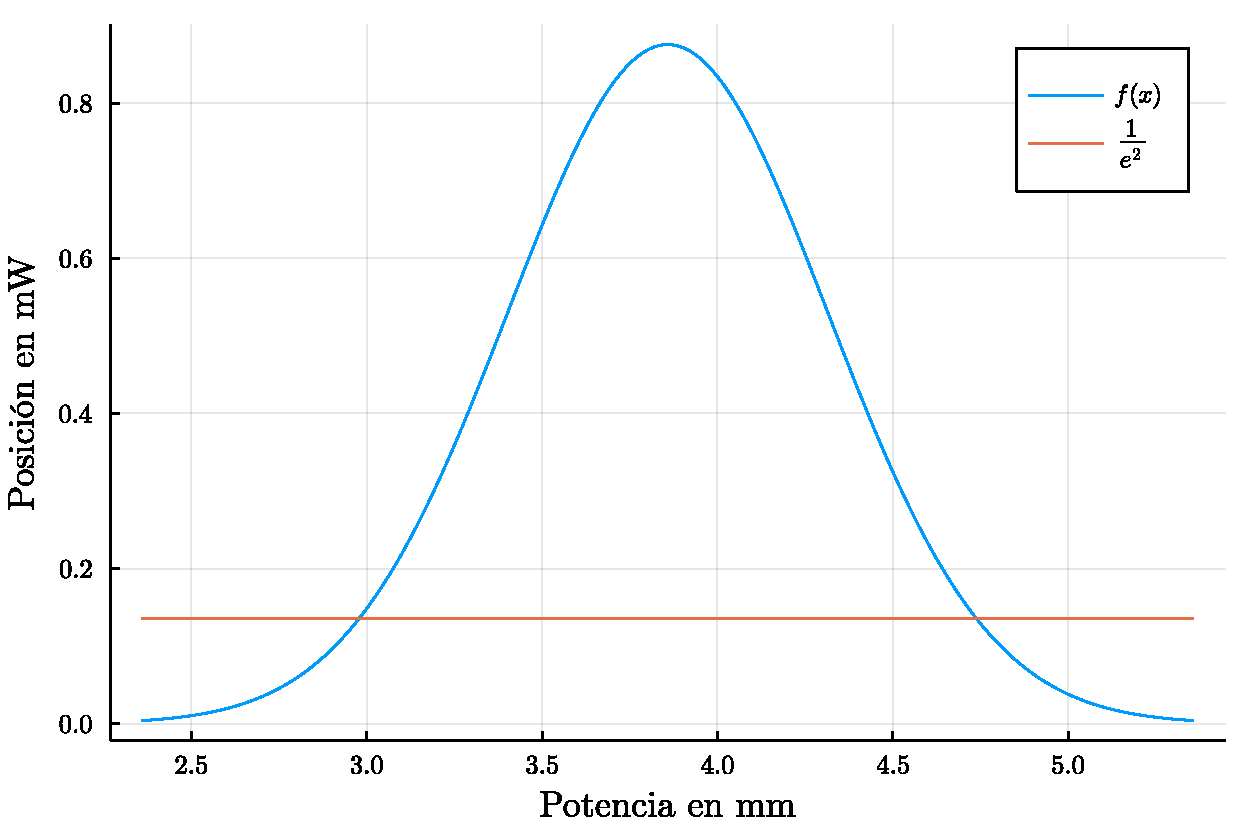
\includegraphics[width=200pt]{img/normal_2.pdf}
			\captionof{figure}{Potencia en función de la posición cruzando $\frac{1}{e^2}$. 1m de distancia.}
		\end{center}

		Las soluciones encontradas y su diferencia fueron las siguientes.

		$$
		x_1=2.9778964
		$$
		$$
		x_2=4.7387398
		$$
		$$
		x_2 - x_1 = 1.7608434
		$$

	\section{Discusión}
		A partir de los resultados anteriores podemos concluir que el tamaño del spot a 30cm es de 0.9952mm y a 1m es de 1.76084mm. A mayor distancia el spot del láser se expande y por lo tanto los resultados están dentro de lo esperado.

\end{document}